\documentclass{beamer}
%Imports and customization
\usepackage{tikz}
\usepackage{graphicx}
\usepackage{tikz-feynman}
\usepackage{ulem}
\usepackage{colortbl}
\graphicspath{ 
    {./images/}
}

\beamertemplatenavigationsymbolsempty
\setbeamertemplate{sidebar right}{}
\setbeamertemplate{footline}{
    \hfill\usebeamertemplate***{navigation symbols}
    \hspace{1cm}\insertframenumber{}/\inserttotalframenumber
}
\setbeamertemplate{caption}{\raggedright\insertcaption\par}
\setbeamersize{text margin left=4mm,text margin right=4mm} 

\setbeamerfont{itemize/enumerate body}{size=\scriptsize}
\setbeamerfont{itemize/enumerate subbody}{size=\scriptsize}
\setbeamerfont{itemize/enumerate subsubbody}{size=\scriptsize}


%Custom Macros
\newcommand{\statwarn}{
    \tiny \color{red} Absolute numbers here mean NOTHING. Plots are based on small (100k events) samples, and are highly biased. All that matters is relative position!
}


% WARNING: When using these commands, the image argument must
% NOT have spaces between itself and the braces
\newcommand{\fullscreenimage}[2]{
    \frame{
        \frametitle{#1} 
        \begin{figure}
        \includegraphics[height=0.9\textheight,width=\textwidth,keepaspectratio]{#2}
        \end{figure}
    }
}


\newcommand{\importpdf}[3]{
    \frame{
        \begin{columns}\column{\dimexpr\paperwidth-10pt}
        \begin{figure}
        \includegraphics[page=#2,height=0.8\textheight,width=\textwidth,keepaspectratio]{#1}
        \end{figure}

        {\tiny #3}
        \end{columns}
    }
}


\newcommand{\displayone}[3]{
    \frame{
        \frametitle{#1} 
        \begin{columns}
            \begin{column}{0.5\textwidth}
                #2
            \end{column}
            \begin{column}{0.5\textwidth}
                \begin{figure}
                    \includegraphics[width=\linewidth,height=\textheight,keepaspectratio]{#3}
                \end{figure}
            \end{column}
        \end{columns}
    }
}

\newcommand{\displayonelarge}[3]{
    \frame{
        \frametitle{#1} 
        \begin{columns}
            \begin{column}{0.3\textwidth}
                #2
            \end{column}
            \begin{column}{0.7\textwidth}
                \begin{figure}
                    \includegraphics[width=\linewidth,height=0.8\textheight,keepaspectratio]{#3}
                \end{figure}
            \end{column}
        \end{columns}
    }
}


\newcommand{\displaytwo}[4]{
    \frame{
        \frametitle{#1} 
        #2
        \begin{columns}
            \begin{column}{0.5\textwidth}
                \begin{figure}
                    \includegraphics[width=\linewidth,height=\textheight,keepaspectratio]{#3}
                \end{figure}
            \end{column}
            \begin{column}{0.5\textwidth}
                \begin{figure}
                    \includegraphics[width=\linewidth,height=\textheight,keepaspectratio]{#4}
                \end{figure}
            \end{column}
        \end{columns}
    }
}

\newcommand{\displaytwocaption}[6]{
    \frame{
        \frametitle{#1} 
        #2
        \begin{columns}
            \begin{column}{0.5\textwidth}
                \begin{figure}
                    \includegraphics[width=\linewidth,height=\textheight,keepaspectratio]{#3}
                    \caption{#4}
                \end{figure}
            \end{column}
            \begin{column}{0.5\textwidth}
                \begin{figure}
                    \includegraphics[width=\linewidth,height=\textheight,keepaspectratio]{#5}
                    \caption{#6}
                \end{figure}
            \end{column}
        \end{columns}
    }
}

\newcommand{\displaytwoVcaption}[6]{
    \frame{
        \begin{columns}
            \begin{column}{0.5\textwidth}
                \frametitle{#1} 
                #2
            \end{column}
            \begin{column}{0.5\textwidth}
                \begin{figure}
                    \includegraphics[width=\linewidth,height=0.3\textheight,keepaspectratio]{#3}
                    \caption{#4}
                \end{figure}

                \begin{figure}
                    \includegraphics[width=\linewidth,height=0.3\textheight,keepaspectratio]{#5}
                    \caption{#6}
                \end{figure}
            \end{column}
        \end{columns}
    }
}


\newcommand{\displaythree}[5]{
    \frame{
        \begin{columns}[T]
            \begin{column}{0.4\textwidth}
                {\usebeamercolor[fg]{title} \insertframetitle{#1} }\\
                \vspace{5mm}
                #2
            \end{column}
            \begin{column}{0.4\textwidth}
                \begin{figure}
                    \includegraphics[width=\linewidth,height=\textheight,keepaspectratio]{#3}
                \end{figure}
            \end{column}
        \end{columns}
        \begin{columns}[T]
            \begin{column}{0.4\textwidth}
                \begin{figure}
                    \includegraphics[width=\linewidth,height=\textheight,keepaspectratio]{#4}
                \end{figure}
            \end{column}
            \begin{column}{0.4\textwidth}
                \begin{figure}
                    \includegraphics[width=\linewidth,height=\textheight,keepaspectratio]{#5}
                \end{figure}
            \end{column}
        \end{columns}
    }
}


\newcommand{\displayfour}[5]{
    \frame{
        \frametitle{#1} 
        \begin{columns}[T]
            \begin{column}{0.4\textwidth}
                \begin{figure}
                    \includegraphics[width=\linewidth,height=\textheight,keepaspectratio]{#2}
                \end{figure}
            \end{column}
            \begin{column}{0.4\textwidth}
                \begin{figure}
                    \includegraphics[width=\linewidth,height=\textheight,keepaspectratio]{#3}
                \end{figure}
            \end{column}
        \end{columns}
        \begin{columns}[T]
            \begin{column}{0.4\textwidth}
                \begin{figure}
                    \includegraphics[width=\linewidth,height=\textheight,keepaspectratio]{#4}
                \end{figure}
            \end{column}
            \begin{column}{0.4\textwidth}
                \begin{figure}
                    \includegraphics[width=\linewidth,height=\textheight,keepaspectratio]{#5}
                \end{figure}
            \end{column}
        \end{columns}
    }
}


\newcommand{\pstrike}[2]{
    \only<-\the\numexpr#1-1>{#2}
    \only<#1->{\sout{#2}}
}


\newcommand{\announcesection}[1]{
    \section{#1}
    \frame{
        \begin{center}
            {\huge #1} 
        \end{center}
    }
}

\newcommand{\kvv}{\kappa_{2V}}
\newcommand{\kl}{\kappa_{\lambda}}
\newcommand{\kv}{\kappa_{V}}

\newcommand{\fkvv}[1]{\kappa_{2V,#1}}
\newcommand{\fkl} [1]{\kappa_{\lambda,#1}}
\newcommand{\fkv} [1]{\kappa_{V,#1}}

\newcommand{\importpdfwpages}[3]{
    \foreach \pageN in {#2,...,#3}{
        \importpdf{#1}{\pageN}{}
    }
}

\newcommand{\hyper}[2]{{\color{blue}\href{#1}{#2}}}



%Begin Presentation
\begin{document}
\title{Work on a New VBF Tagging Algorithm}
\author{Chris Milke}
\date{8 December, 2019}

\frame{\titlepage}
\frame{\frametitle{Overview} \tableofcontents}





\section{Background}

\frame{
    \frametitle{ Offline to Online: The B-Jet Trigger Retuning Process }
    \begin{figure}
        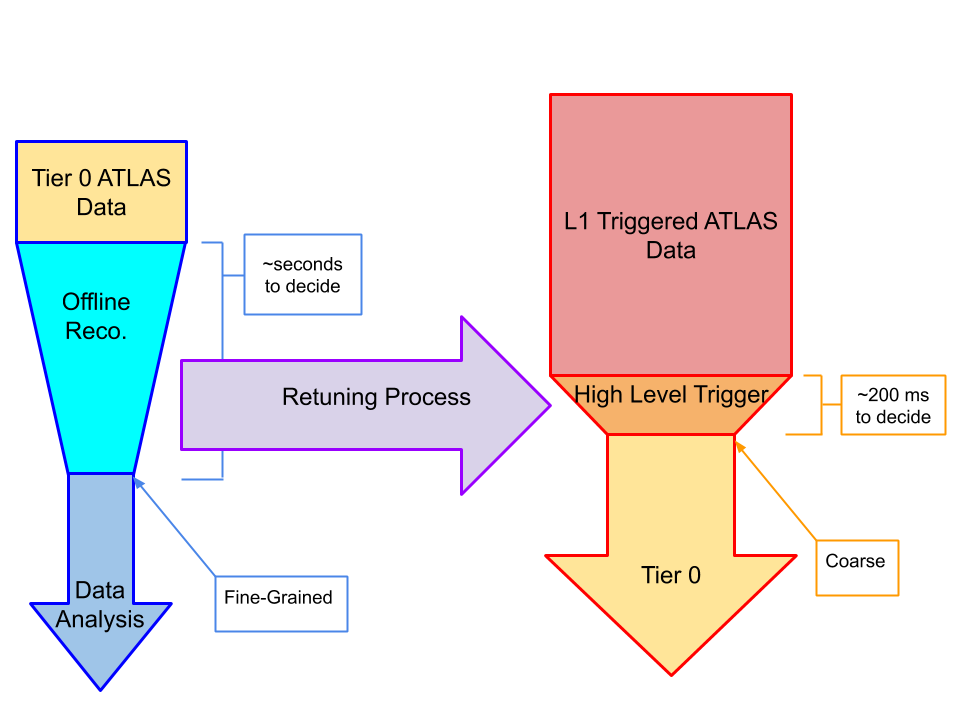
\includegraphics[width=\linewidth,height=\textheight,keepaspectratio]{offline_to_online}
    \end{figure}
}


\frame{
    \frametitle{ Details of the Retuning Process }
    \begin{figure}
        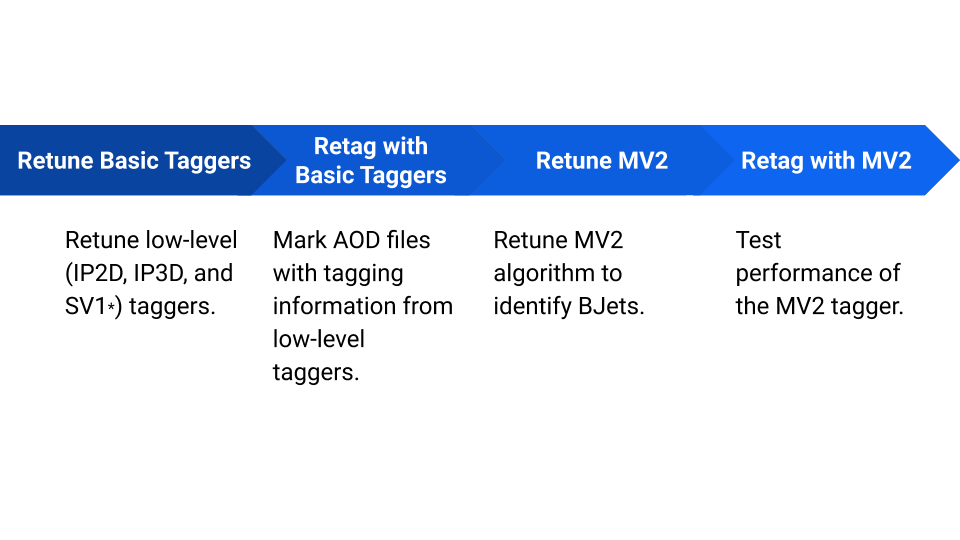
\includegraphics[width=\linewidth,height=\textheight,keepaspectratio]{retune_process}
    \end{figure}
}
 %TODO
%%Slides like peilong’s slide 3 and 4 (about event generation and selection mechanisms

%Show eta distributions, then show that gamma plot that shows the gap in photon coverage from tight/loose photon (as explanation for why I filter on truth photons)





%\displaythree{Comparison of $d_0$}
%    { \begin{itemize}
%        \item Used for IP2D
%        \item Significance is what is ultimately used in tagging
%        \item Significance = $d_0$ / error
%        \item $d_0$ Error for FTK-IDTrig appears "shifted"
%    \end{itemize} }
%    {track_study/plot_d0_0}
%    {track_study/plot_d0_err_0}
%    {track_study/plot_d0_sig_0}
%\displaythree{Comparison of $z_0\sin\theta$}
%    { \begin{itemize}
%        \item Used for IP3D
%        \item Base value looks similar again
%        \item Shape of the errors distribution even more distinctive from HLT
%    \end{itemize} }
%    {track_study/plot_z0sintheta_0}
%    {track_study/plot_z0sintheta_err_0}
%    {track_study/plot_z0sintheta_sig_0}
 %TODO
\announcesection{Algorithm Performance} 

\displayonelarge{Invariant Mass as a Discriminating Variable}
    { \footnotesize
        Choose two ``VBF Jets",
        then use their invariant mass
        as a discriminant in tagging.
    }
    {remote/figures/fig_mjj_null_mjj_distribution.pdf}


\displayonelarge{Performance Curves: Baseline}
    {Performance of $M_{jj}$ discriminant for events with two jets is not unreasonable.}
    {remote/performance/focused_perf_2only_roc_efficiency.pdf}

\displayonelarge{Performance Curves: Dealing with Three Jets}
    { \footnotesize
        With three jets, we need to decide which two are the VBF signal jets, and use these to calculate the $M_{jj}$ discriminant.

        \vspace{5mm}

        Naively, we can try picking the two leading $p_t$ jets. This drastically reduces performance.
    }
    {remote/performance/focused_perf_2-pt_roc_efficiency.pdf}

\displayonelarge{\small Two Measures of Performance: Tagging Efficiency VS Selection Efficiency}
    { \footnotesize
        Why do the leading $p_t$ jets perform so badly?

        \vspace{5mm}

        ...Well, how often are the leading $p_t$ jets actually the VBF jets?

        \vspace{5mm}

        \begin{tabular}{|c|c|}\hline
        Algorithm & Efficiency \\
        \hline
        Leading $p_t$ & 53\% \\
        \hline
        \end{tabular}
    }
    {remote/performance/focused_perf_2-pt_roc_efficiency.pdf}

\displayonelarge{Performance Curves: Worst Case Scenario}
    { \footnotesize
        How closely is selection efficiency related to tagging efficiency?

        Let's look at a worst case situation:
        What if the "VBF Jets" were chosen at random?

        \vspace{5mm}

        \begin{tabular}{|c|c|}\hline
        Algorithm & Efficiency \\ \hline
        Leading $p_t$ & 53\% \\ \hline
        Random & 33\% \\ \hline
        \end{tabular}
    }
    {remote/performance/focused_perf_2-pt-R_roc_efficiency.pdf}

\displayonelarge{Performance Curves: Best Case Scenario}
    { \footnotesize
        What about perfect selection efficiency?

        {\tiny CAUTION: Truth selection treats signal and background events \textit{differently};
        it is biasing the tagging performance and should be viewed only as an estimate}

        \vspace{5mm}

        \begin{tabular}{|c|c|}\hline
        Algorithm & Efficiency \\ \hline
        Leading $p_t$ & 53\% \\ \hline
        Random & 33\% \\ \hline
        Truth & 100\% \\ \hline
        \end{tabular}
    }
    {remote/performance/focused_perf_2-pt-R-T_roc_efficiency.pdf}

\displayonelarge{Performance Curves: A Better Approach}
    { \footnotesize
        A smarter approach is to use the jet pair which maximizes $M_{jj}$

        \vspace{5mm}

        \begin{tabular}{|c|c|}\hline
        Algorithm & Efficiency \\ \hline
        Leading $p_t$ & 53\% \\ \hline
        Random & 33\% \\ \hline
        Truth & 100\% \\ \hline
        Max $M_{jj}$& 66\% \\ \hline
        \end{tabular}
    }
    {remote/performance/focused_perf_2-pt-R-T-mjj_roc_efficiency.pdf}

\displayonelarge{Performance Curves: Introduce Machine Learning}
    { \footnotesize
        Enter Machine Learning... which seems to just be replicating $M_{jj}$ right now.
        I'm investigating ways to improve it.

        \vspace{5mm}

        \begin{tabular}{|c|c|}\hline
        Algorithm & Efficiency \\ \hline
        Leading $p_t$ & 53\% \\ \hline
        Random & 33\% \\ \hline
        Truth & 100\% \\ \hline
        Max $M_{jj}$ & 66\% \\ \hline
        MLP & 66\% \\ \hline
        \end{tabular}
    }
    {remote/performance/focused_perf_2-pt-R-T-mjj-mlp_roc_efficiency.pdf}

\displayonelarge{Performance Curves: What About a Better Tagger?}
    { \footnotesize
        A machine-learning-based tagger easily outperforms the $M_{jj}$-based tagger.

        \vspace{5mm}

        \begin{tabular}{|c|c|}\hline
        Algorithm & Efficiency \\ \hline
        Leading $p_t$ & 53\% \\ \hline
        Random & 33\% \\ \hline
        Truth & 100\% \\ \hline
        Max $M_{jj}$ & 66\% \\ \hline
        MLP & 66\% \\ \hline
        \end{tabular}
    }
    {remote/performance/focused_perf_2-mjj-mlp_NN_roc_efficiency.pdf}

\displayonelarge{Performance Curves: Overall Performance}
    {
        If we look at the combined performance of 2 and 3 jet events,
        the difference is not dramatic, but there is still room for improvement.

    }
    {remote/performance/focused_perf_2-3-summary_roc_efficiency.pdf}
 %TODO
%\section{Continuing Work}
\frame {
    \frametitle{Continuing Work}
    \begin{itemize} {
        \item Learn how to improve machine learning architecture
        \item Learn details of ``third jet", and how to distinguish ISR from FSR
    } \end{itemize}
}
 %TODO

\section{Conclusion} %TODO
%\frame{
%    \frametitle{Conclusions}
%    \begin{itemize} {\normalsize
%        \item FTK tracks, even with retuning,
%            lead to less light-jet rejection in flavour tagging
%            compared to the HLT-only counterpart
%        \item We want to understand the exact reasons for the observed gap in performance
%        \item Comparing track parameters jet-by-jet,
%            primary cause appears to be FTK-IDTrig's lower tolerance to small values of d0
%        \item This may be related to the apparent "shift" in d0-error. More studies needed
%        \item Track quality values seem to be irrelevant to B-Tagging performance
%        \item Additional studies are ongoing. Comments and ideas are welcome
%    } \end{itemize}
%}

\announcesection{Backup}
\frame {
    \frametitle{Existing VBF Tagging Methods}

   % I'm having a hard time finding anything in papers that I can compare to my own methods.
   % They all use "acceptance", which is the algorithm efficiency x the % of events that pass the event selection criteria.

   %Maybe try to grab the presentation Katherine sent your way

    %WHY??: Look at the various analyses you’ve found, and show the inefficiencies they work with that I hope to improve
        %VBF->H->gam-gam (relies on gam-gam tagging)
        %VBF->H->BBbar (relies on btagging)
        %VBF->H->Invis

}


\fullscreenimage{VBF->H->$\gamma\gamma$ Kinematic Selections}{vbf-H-gamgam_kinematic_region.png}
 %TODO
\end{document}
